\documentclass[10pt,a4paper]{article}\usepackage[]{graphicx}\usepackage[]{color}
%% maxwidth is the original width if it is less than linewidth
%% otherwise use linewidth (to make sure the graphics do not exceed the margin)
\makeatletter
\def\maxwidth{ %
  \ifdim\Gin@nat@width>\linewidth
    \linewidth
  \else
    \Gin@nat@width
  \fi
}
\makeatother

\definecolor{fgcolor}{rgb}{0.345, 0.345, 0.345}
\newcommand{\hlnum}[1]{\textcolor[rgb]{0.686,0.059,0.569}{#1}}%
\newcommand{\hlstr}[1]{\textcolor[rgb]{0.192,0.494,0.8}{#1}}%
\newcommand{\hlcom}[1]{\textcolor[rgb]{0.678,0.584,0.686}{\textit{#1}}}%
\newcommand{\hlopt}[1]{\textcolor[rgb]{0,0,0}{#1}}%
\newcommand{\hlstd}[1]{\textcolor[rgb]{0.345,0.345,0.345}{#1}}%
\newcommand{\hlkwa}[1]{\textcolor[rgb]{0.161,0.373,0.58}{\textbf{#1}}}%
\newcommand{\hlkwb}[1]{\textcolor[rgb]{0.69,0.353,0.396}{#1}}%
\newcommand{\hlkwc}[1]{\textcolor[rgb]{0.333,0.667,0.333}{#1}}%
\newcommand{\hlkwd}[1]{\textcolor[rgb]{0.737,0.353,0.396}{\textbf{#1}}}%

\usepackage{framed}
\makeatletter
\newenvironment{kframe}{%
 \def\at@end@of@kframe{}%
 \ifinner\ifhmode%
  \def\at@end@of@kframe{\end{minipage}}%
  \begin{minipage}{\columnwidth}%
 \fi\fi%
 \def\FrameCommand##1{\hskip\@totalleftmargin \hskip-\fboxsep
 \colorbox{shadecolor}{##1}\hskip-\fboxsep
     % There is no \\@totalrightmargin, so:
     \hskip-\linewidth \hskip-\@totalleftmargin \hskip\columnwidth}%
 \MakeFramed {\advance\hsize-\width
   \@totalleftmargin\z@ \linewidth\hsize
   \@setminipage}}%
 {\par\unskip\endMakeFramed%
 \at@end@of@kframe}
\makeatother

\definecolor{shadecolor}{rgb}{.97, .97, .97}
\definecolor{messagecolor}{rgb}{0, 0, 0}
\definecolor{warningcolor}{rgb}{1, 0, 1}
\definecolor{errorcolor}{rgb}{1, 0, 0}
\newenvironment{knitrout}{}{} % an empty environment to be redefined in TeX

\usepackage{alltt}
\usepackage[latin1]{inputenc}
\usepackage{amsmath}
\usepackage{amsfonts}
\usepackage{amssymb}
\author{Erika Martínez}
\title{Guías prácticas}
\IfFileExists{upquote.sty}{\usepackage{upquote}}{}
\begin{document}

\maketitle
\newpage

Pr?ctica 10-An?lisis de una variable bidimensional (categ?rica, continua)

EJEMPLO 1
Crea un vector de datos para cada proceso descrito en el problema. 
\begin{knitrout}
\definecolor{shadecolor}{rgb}{0.969, 0.969, 0.969}\color{fgcolor}\begin{kframe}
\begin{alltt}
\hlstd{A} \hlkwb{<-} \hlkwd{c}\hlstd{(}\hlnum{100}\hlstd{,}\hlnum{96}\hlstd{,}\hlnum{92}\hlstd{,}\hlnum{96}\hlstd{,}\hlnum{92}\hlstd{); A}
\end{alltt}
\begin{verbatim}
## [1] 100  96  92  96  92
\end{verbatim}
\begin{alltt}
\hlstd{B} \hlkwb{<-} \hlkwd{c}\hlstd{(}\hlnum{76}\hlstd{,}\hlnum{80}\hlstd{,}\hlnum{75}\hlstd{,}\hlnum{84}\hlstd{,}\hlnum{82}\hlstd{); B}
\end{alltt}
\begin{verbatim}
## [1] 76 80 75 84 82
\end{verbatim}
\begin{alltt}
\hlstd{C} \hlkwb{<-} \hlkwd{c}\hlstd{(}\hlnum{108}\hlstd{,}\hlnum{100}\hlstd{,}\hlnum{96}\hlstd{,}\hlnum{98}\hlstd{,}\hlnum{100}\hlstd{); C}
\end{alltt}
\begin{verbatim}
## [1] 108 100  96  98 100
\end{verbatim}
\end{kframe}
\end{knitrout}


Crea una hoja de datos teniendo como componentes (columnas) los tres vectores
\begin{knitrout}
\definecolor{shadecolor}{rgb}{0.969, 0.969, 0.969}\color{fgcolor}\begin{kframe}
\begin{alltt}
\hlstd{Baterias} \hlkwb{<-} \hlkwd{data.frame}\hlstd{(}\hlkwc{procesoA}\hlstd{=A,} \hlkwc{procesoB}\hlstd{=B,} \hlkwc{procesoC}\hlstd{=C); Baterias}
\end{alltt}
\begin{verbatim}
##   procesoA procesoB procesoC
## 1      100       76      108
## 2       96       80      100
## 3       92       75       96
## 4       96       84       98
## 5       92       82      100
\end{verbatim}
\end{kframe}
\end{knitrout}

 Para editar los datos puede utilizar la funci?n fix() 
\begin{knitrout}
\definecolor{shadecolor}{rgb}{0.969, 0.969, 0.969}\color{fgcolor}\begin{kframe}
\begin{alltt}
\hlkwd{fix}\hlstd{(Baterias)}
\end{alltt}
\end{kframe}
\end{knitrout}

Guarda la hoja de datos en un archivo. 
\begin{knitrout}
\definecolor{shadecolor}{rgb}{0.969, 0.969, 0.969}\color{fgcolor}\begin{kframe}
\begin{alltt}
\hlkwd{write.table}\hlstd{(Baterias,} \hlkwc{file}\hlstd{=}\hlstr{"Baterias.txt"}\hlstd{,} \hlkwc{append}\hlstd{=}\hlnum{FALSE}\hlstd{,} \hlkwc{quote}\hlstd{=}\hlnum{TRUE}\hlstd{,} \hlkwc{sep}\hlstd{=}\hlstr{" "}\hlstd{,}
\hlkwc{na}\hlstd{=}\hlstr{"NA"}\hlstd{,} \hlkwc{col.names}\hlstd{=}\hlnum{TRUE}\hlstd{)}
\end{alltt}
\end{kframe}
\end{knitrout}

Elimina todos objetos que existen en el espacio de trabajo (Workspace) 
\begin{knitrout}
\definecolor{shadecolor}{rgb}{0.969, 0.969, 0.969}\color{fgcolor}\begin{kframe}
\begin{alltt}
\hlkwd{ls}\hlstd{();} \hlkwd{rm}\hlstd{(}\hlkwc{list}\hlstd{=}\hlkwd{ls}\hlstd{(}\hlkwc{all}\hlstd{=}\hlnum{TRUE}\hlstd{));} \hlkwd{ls}\hlstd{()}
\end{alltt}
\begin{verbatim}
## [1] "A"        "B"        "Baterias" "C"
## character(0)
\end{verbatim}
\end{kframe}
\end{knitrout}

Recupera la hoja de datos,para probar si fue guardada. 
\begin{knitrout}
\definecolor{shadecolor}{rgb}{0.969, 0.969, 0.969}\color{fgcolor}\begin{kframe}
\begin{alltt}
\hlstd{Baterias} \hlkwb{<-} \hlkwd{read.table}\hlstd{(}\hlstr{"Baterias.txt"}\hlstd{,} \hlkwc{header}\hlstd{=}\hlnum{TRUE}\hlstd{); Baterias}
\end{alltt}
\begin{verbatim}
##   procesoA procesoB procesoC
## 1      100       76      108
## 2       96       80      100
## 3       92       75       96
## 4       96       84       98
## 5       92       82      100
\end{verbatim}
\end{kframe}
\end{knitrout}

\begin{knitrout}
\definecolor{shadecolor}{rgb}{0.969, 0.969, 0.969}\color{fgcolor}\begin{kframe}
\begin{alltt}
\hlcom{#Conecta o adjunta la hoja de datos a la segunda ruta o lista de b?squeda. }
\hlkwd{attach}\hlstd{(Baterias,} \hlkwc{pos}\hlstd{=}\hlnum{2}\hlstd{)}
\hlkwd{search}\hlstd{()}
\end{alltt}
\begin{verbatim}
##  [1] ".GlobalEnv"        "Baterias"          "package:knitr"    
##  [4] "package:stats"     "package:graphics"  "package:grDevices"
##  [7] "package:utils"     "package:datasets"  "package:methods"  
## [10] "Autoloads"         "package:base"
\end{verbatim}
\begin{alltt}
\hlcom{#Dibuja un gr?fico horizontal depuntos para los tres procesos. }
\hlkwd{stripchart}\hlstd{(Baterias,} \hlkwc{main}\hlstd{=}\hlstr{"Gr?fico de puntos para los tres procesos"}\hlstd{,}
\hlkwc{method} \hlstd{=} \hlstr{"stack"}\hlstd{,} \hlkwc{vertical} \hlstd{=} \hlnum{FALSE}\hlstd{,} \hlkwc{col}\hlstd{=}\hlstr{"blue"}\hlstd{,} \hlkwc{pch}\hlstd{=}\hlnum{1}\hlstd{,} \hlkwc{xlab}\hlstd{=}\hlstr{"Duraci?n (semanas)"}\hlstd{,} \hlkwc{ylab}\hlstd{=}\hlstr{"Proceso"}\hlstd{)}
\end{alltt}
\end{kframe}
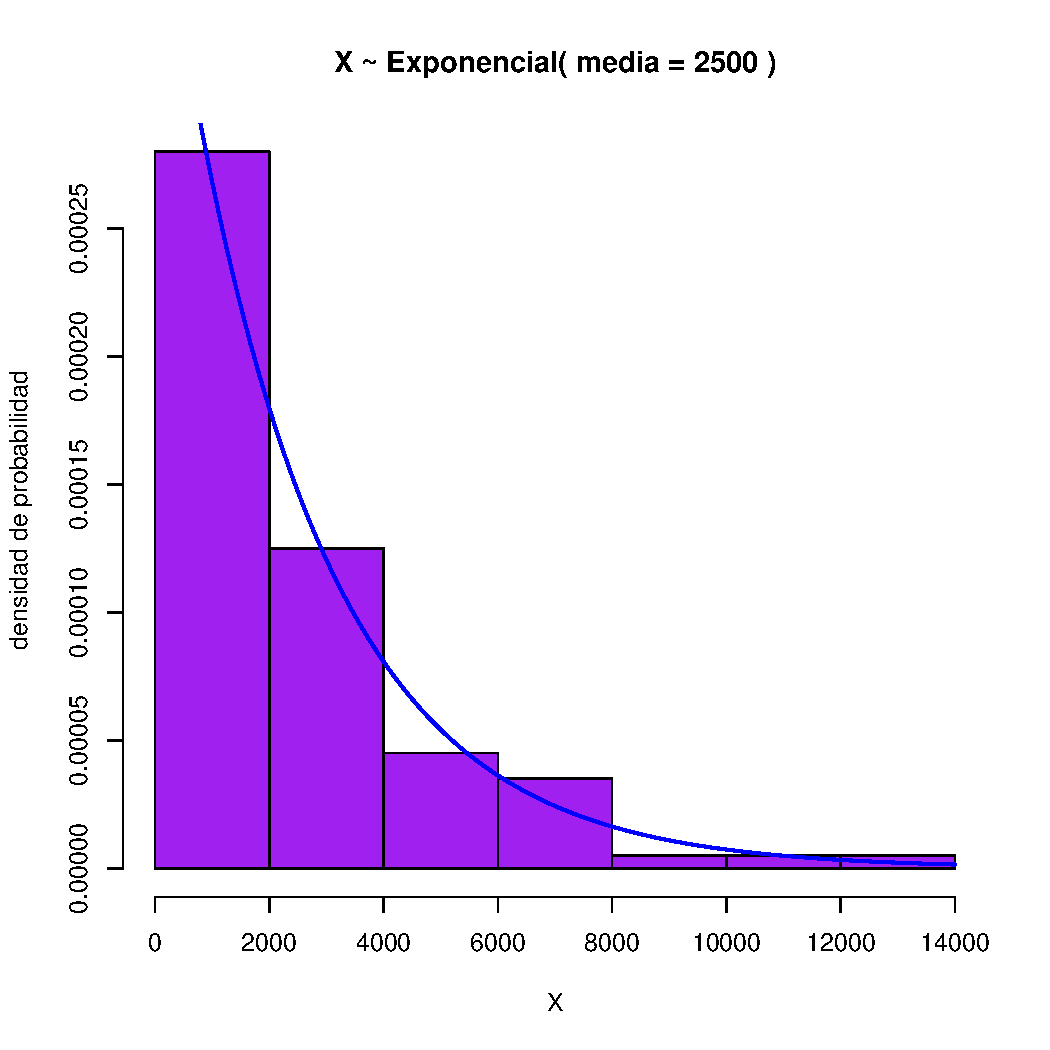
\includegraphics[width=\maxwidth]{figure/unnamed-chunk-7-1} 
\begin{kframe}\begin{alltt}
\hlcom{#Muestra un resumen estad?stico para los tres procesos. }
\hlkwd{summary}\hlstd{(Baterias)}
\end{alltt}
\begin{verbatim}
##     procesoA        procesoB       procesoC    
##  Min.   : 92.0   Min.   :75.0   Min.   : 96.0  
##  1st Qu.: 92.0   1st Qu.:76.0   1st Qu.: 98.0  
##  Median : 96.0   Median :80.0   Median :100.0  
##  Mean   : 95.2   Mean   :79.4   Mean   :100.4  
##  3rd Qu.: 96.0   3rd Qu.:82.0   3rd Qu.:100.0  
##  Max.   :100.0   Max.   :84.0   Max.   :108.0
\end{verbatim}
\begin{alltt}
\hlcom{#Dibuja un gr?fico horizontal de cajas (box-plot) para los tres procesos. }
\hlkwd{boxplot}\hlstd{(Baterias,} \hlkwc{width}\hlstd{=}\hlkwa{NULL}\hlstd{,} \hlkwc{varwidth}\hlstd{=}\hlnum{TRUE}\hlstd{,names,} \hlkwc{add}\hlstd{=} \hlnum{FALSE}\hlstd{,} \hlkwc{horizontal} \hlstd{=} \hlnum{TRUE}\hlstd{,}
\hlkwc{main}\hlstd{=}\hlstr{"Gr?fico de caja por proceso"}\hlstd{,} \hlkwc{border}\hlstd{=}\hlkwd{par}\hlstd{(}\hlstr{"fg"}\hlstd{),} \hlkwc{col}\hlstd{=}\hlkwd{c}\hlstd{(}\hlstr{"blue"}\hlstd{,} \hlstr{"black"}\hlstd{,} \hlstr{"purple"}\hlstd{),} \hlkwc{xlab} \hlstd{=}
\hlstr{"Duraci?n (semanas)"}\hlstd{,} \hlkwc{ylab}\hlstd{=}\hlstr{"Proceso"}\hlstd{)}
\end{alltt}
\end{kframe}
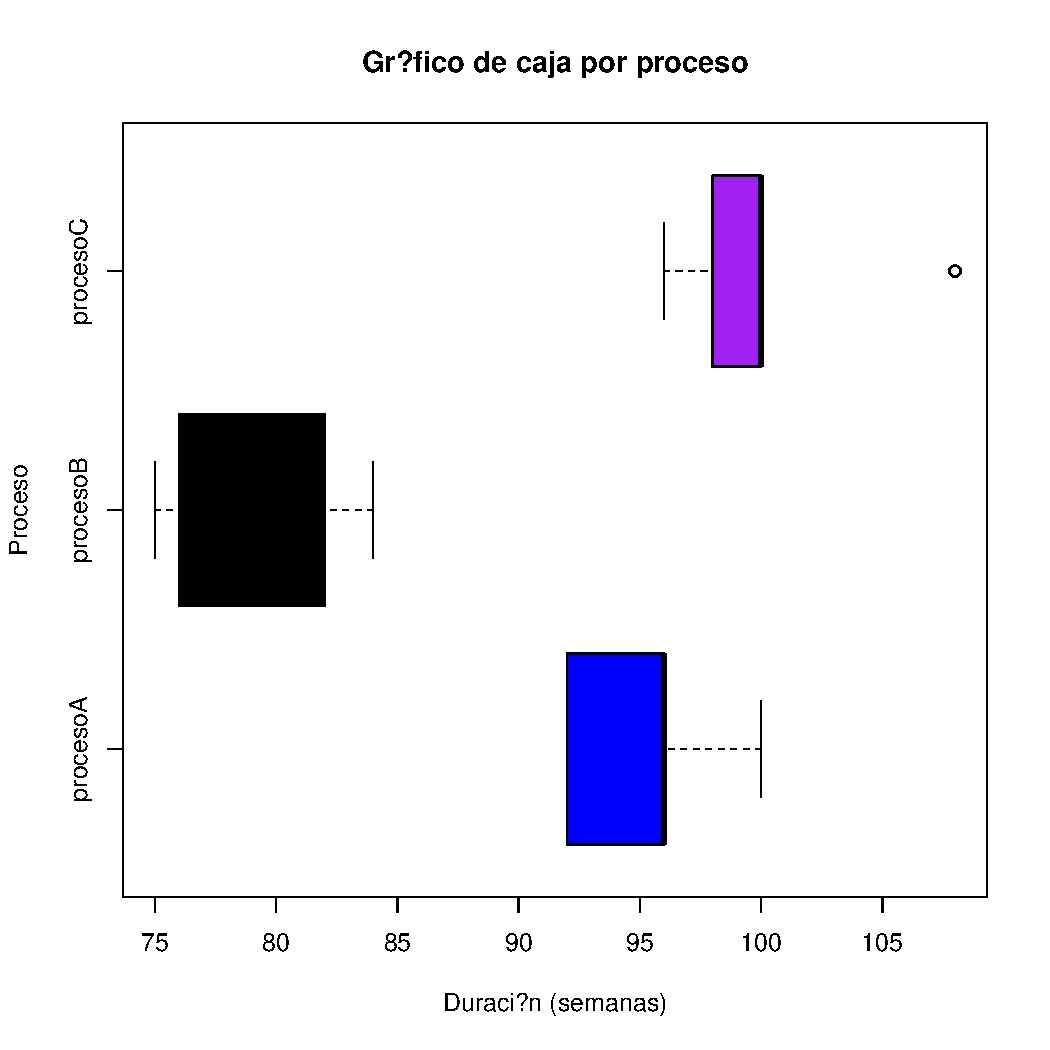
\includegraphics[width=\maxwidth]{figure/unnamed-chunk-7-2} 

\end{knitrout}

\begin{knitrout}
\definecolor{shadecolor}{rgb}{0.969, 0.969, 0.969}\color{fgcolor}\begin{kframe}
\begin{alltt}
\hlcom{# Vertical }
\hlkwd{boxplot}\hlstd{(Baterias,} \hlkwc{width}\hlstd{=}\hlkwa{NULL}\hlstd{,} \hlkwc{varwidth}\hlstd{=}\hlnum{TRUE}\hlstd{,names,} \hlkwc{add}\hlstd{=} \hlnum{FALSE}\hlstd{,} \hlkwc{horizontal} \hlstd{=} \hlnum{FALSE}\hlstd{,}
\hlkwc{main}\hlstd{=}\hlstr{"Gr?fico de caja por proceso"}\hlstd{,} \hlkwc{border}\hlstd{=}\hlkwd{par}\hlstd{(}\hlstr{"fg"}\hlstd{),} \hlkwc{col}\hlstd{=}\hlkwd{c}\hlstd{(}\hlstr{"bluen"}\hlstd{,} \hlstr{"purple"}\hlstd{,} \hlstr{"black"}\hlstd{),} \hlkwc{xlab} \hlstd{=}
\hlstr{"Duraci?n (semanas)"}\hlstd{,} \hlkwc{ylab}\hlstd{=}\hlstr{"Proceso"}\hlstd{)}
\end{alltt}


{\ttfamily\noindent\bfseries\color{errorcolor}{\#\# Error in xypolygon(xx, yy, lty = "{}blank"{}, col = boxfill[i]): invalid color name 'bluen'}}\end{kframe}

\includegraphics[width=\maxwidth]{figure/unnamed-chunk-8-1} 
\begin{kframe}\begin{alltt}
\hlcom{#Presenta la matriz de covarianzas muestral. }
\hlkwd{options}\hlstd{(}\hlkwc{digits}\hlstd{=}\hlnum{3}\hlstd{)}
\hlstd{S} \hlkwb{<-} \hlkwd{var}\hlstd{(Baterias); S}
\end{alltt}
\begin{verbatim}
##          procesoA procesoB procesoC
## procesoA     11.2     -1.6     12.4
## procesoB     -1.6     14.8     -4.7
## procesoC     12.4     -4.7     20.8
\end{verbatim}
\begin{alltt}
\hlcom{#Presenta la desviaci?n est?ndar de cada proceso. }
\hlcom{#desv <- sd(Baterias); desv}

\hlcom{# Concatena los tres vectores dentro de un vector simple, junto con un vector factor indicador de }
\hlcom{#la categor?a o tratamiento (A, B, C) que origina cada observaci?n.}
\hlstd{Baterias} \hlkwb{<-} \hlkwd{stack}\hlstd{(Baterias); Baterias}
\end{alltt}
\begin{verbatim}
##    values      ind
## 1     100 procesoA
## 2      96 procesoA
## 3      92 procesoA
## 4      96 procesoA
## 5      92 procesoA
## 6      76 procesoB
## 7      80 procesoB
## 8      75 procesoB
## 9      84 procesoB
## 10     82 procesoB
## 11    108 procesoC
## 12    100 procesoC
## 13     96 procesoC
## 14     98 procesoC
## 15    100 procesoC
\end{verbatim}
\end{kframe}
\end{knitrout}

\begin{knitrout}
\definecolor{shadecolor}{rgb}{0.969, 0.969, 0.969}\color{fgcolor}\begin{kframe}
\begin{alltt}
\hlcom{# Prueba de igualdad de medias por descomposici?n de la varianza en dos fuentes de variaci?n:}
\hlstd{aov.Baterias} \hlkwb{<-} \hlkwd{aov}\hlstd{(values}\hlopt{~}\hlstd{ind,} \hlkwc{data}\hlstd{=Baterias)}

\hlcom{# Prueba de igualdad de medias en un dise?o de una v?a}
\hlkwd{oneway.test}\hlstd{(values}\hlopt{~}\hlstd{ind,} \hlkwc{data}\hlstd{=Baterias,} \hlkwc{var.equal} \hlstd{=} \hlnum{TRUE}\hlstd{)}
\end{alltt}
\begin{verbatim}
## 
## 	One-way analysis of means
## 
## data:  values and ind
## F = 40, num df = 2, denom df = 10, p-value = 6e-06
\end{verbatim}
\begin{alltt}
\hlcom{#Deshace la concatenaci?n del vector de valores y el vector indicador de categor?a. }
\hlstd{Baterias} \hlkwb{=} \hlkwd{unstack}\hlstd{(Baterias);Baterias}
\end{alltt}
\begin{verbatim}
##   procesoA procesoB procesoC
## 1      100       76      108
## 2       96       80      100
## 3       92       75       96
## 4       96       84       98
## 5       92       82      100
\end{verbatim}
\begin{alltt}
\hlcom{#Desconecta la hoja de datos de la segunda ruta o lista de b?squeda. }
\hlkwd{detach}\hlstd{(Baterias,} \hlkwc{pos}\hlstd{=}\hlnum{2}\hlstd{);} \hlkwd{search}\hlstd{()}
\end{alltt}
\begin{verbatim}
##  [1] ".GlobalEnv"        "package:knitr"     "package:stats"    
##  [4] "package:graphics"  "package:grDevices" "package:utils"    
##  [7] "package:datasets"  "package:methods"   "Autoloads"        
## [10] "package:base"
\end{verbatim}
\end{kframe}
\end{knitrout}



\end{document}
